The solution is done by dividing the state machine into a FSMD as shown in figure~\ref{fig:fsmd} in appendix~\ref{app:figures} and attaching a datapath

\subsection{The individual states}
we are using nine different states for our logic, each of them implemented in order to fulfil the requirements.
\subsubsection{reset}
The first one is the reset state, where we start from on power on and go to on a hard reset. This state takes care of setting the up the cost and
then "count up" the internal coin counters CC1 and CC2. In a real machine this could be done by a separate processor or circuit (weighing all coins
and deciding by the weight of one coin) outputting this count on a bus. This processor/circuit could also be shut down in all other states but the 
reset state to preserve power. This state automatically jumps to init on the next clock rising edge.\\
Note that the VHDL code differs slightly from the FSM in the this state, as it does not use a register. This was not prioritized, but can be added relatively simple later on.

\subsubsection{init}
This is the initialization state that takes care of everything that has to be done prior to a purchase. This goes directly to the purchase state on the next clock.

\subsubsection{purchase}
This is the main state for doing transactions. The user operating the vending machine is being put back to this state as long as he/she has not inserted enough
money. The state also responds to coin inputs and goes to the relevant states (add1 and add2). When the return\_change button is pressed, we go
to the return\_all state corresponding to requirement 8. We also go to this state if the machine is unable to return change. This is detected by
the datapath and given by the boolean expression show on the transition between purchase and return\_all in figure~\ref{fig:fsmd} (appendix~\ref{app:figures}). This corresponds to requirement 10. Note that we in the FSMD also check if TCC1 is zero. This enables us to detect if 
a user has inserted 8 kr using 2,4 or 6 1 kr and ending with a 2 kr. In this case the machine actually holds change, but we need to do more in order
to make this work - to be continued.\\
\\
When the user has inserted enough money, we move to the merge\_counters state. The logic is shown in figure~\ref{fig:fsm} in appendix~\ref{app:figures}.\\
\\
No assignments are done here as it is not needed.

\subsubsection{add1}
When 1 kr has been inserted into the machine, this state is reached. It counts up the TCC1 register by enabling it and setting the multiplexer to the corresponding value. This is illustrated in figure~\ref{fig:datapath} in appendix~\ref{app:figures}. On the next clock we return to the purchase state.\\
\\
One problem with this is that we have to wait for the machine to return to the purchase state to be able to receive more coin inputs. This will not pose a problem if we have a relatively fast clock, but in our case, with the manual clock, it does. It ``throws away'' coin inputs done in the add1 or add2 state. This problem is discussed in section~\ref{sec:implementation_issues}

\subsubsection{add2}
This is similar to the kr1 state. It just adds to the TCC2 register instead.

\subsubsection{return\_all}
This state simply clears the TCC1 and TCC2 registers (symbolizing a coin return), sets the returned\_all\_coins register high and goes the wait\_for\_user state.


\subsubsection{return\_change}
This state sets the returned\_changed register, decrements CC1 by one and goes to the dispense state.

\subsubsection{merge\_counter}
This is a state that was added relatively late in the process. Our original design was to merge the coin counters in the wait\_for\_user state, but this did not work. This was caused by the fact that we cycled the wait\_for\_user state while the user did not press then purchase\_finished button. As a result, our counters were merged on every clock rising edge. This was no problem with a manual clock, as you could just not clock, but with a clock of just 5Hz the counters would be merged 5 times every second.\\
\\
The solution was to go to a merge state that adds TCC1 with CC1 and TCC2 with CC2 before dispensing. We still have our amount\_eq\_cost and amount\_gt\_cost to guide ud to either the dispense or  the return\_change state.\\
By merging these counters before returning change we complete the case described in purchase section, as we are sure we have change (either CC1 or TCC1 holds a 1 kr), we can go directly to the return\_change state.



\subsubsection{dispense}
This state releases the can and closes the coin slot. These are both D-flip-flops

\subsubsection{wait\_for\_user}
Here we just wait for the user to take the item. Otherwise the machine would go back to init, and purchase too fast for the user too see on a fast clock.\\
This state eventually goes to back init, and the process can start again.

\begin{figure}
\centering
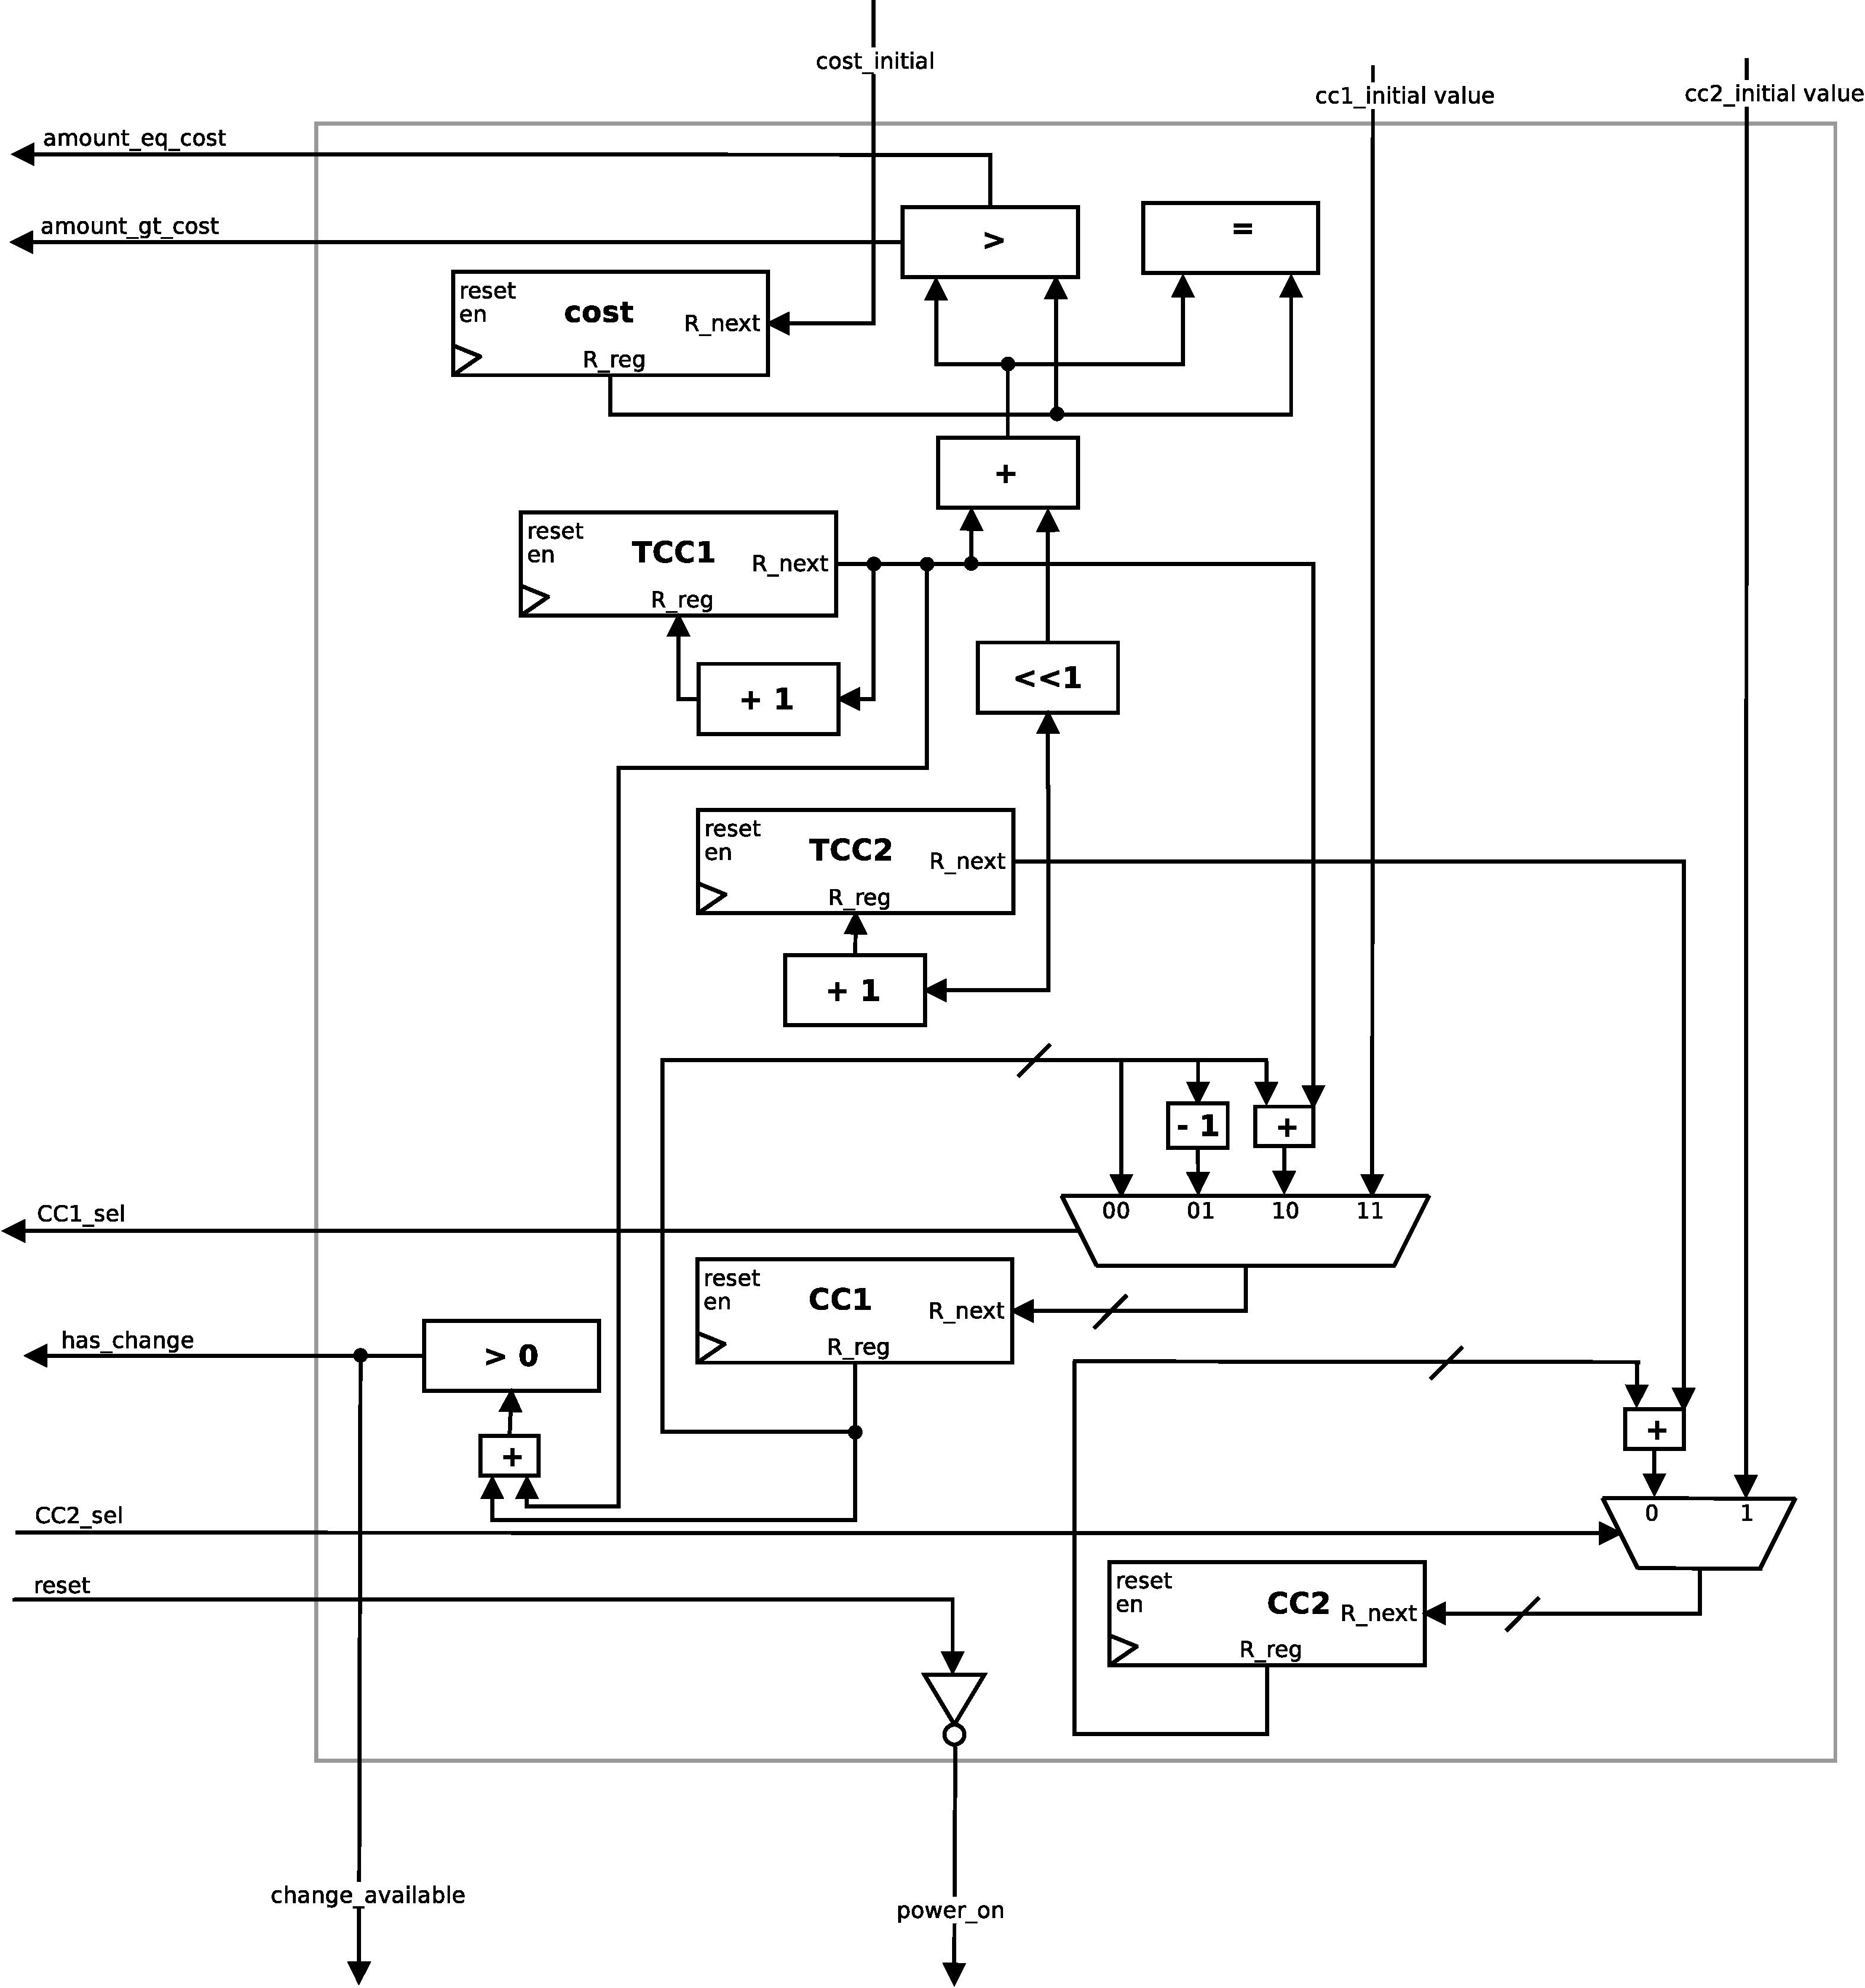
\includegraphics[width=0.8\textwidth]{fig/datapath.pdf}
\caption{Datapath of the processesor (larger version can found in appendix~\ref{app:figures})}
\label{fig:datapath_small}
\end{figure}

\subsection{Datapath}

By putting some of the logic into a datapath we can distinguish the state logic from the calculations. By doing this we were also also able to trim down on our design.
\subsubsection{Cutting the fat}
In a early implementation we had a amount register. This was trivial and involved a lot of housekeeping on it. When designing the datapath we realized that we could do without, as the only things we were really interested in could be calculated on the fly using our TCC1 and TCC2 registers. By left shifting the TCC2 register and adding it with the TCC1 register we now had a bus containing the current amount. Getting the amount\_gt\_cost and amount\_eq\_cost was now just a matter of doing simple comparisons on the bus and the cost register.
\subsubsection{debug}
\label{sec:debug}
The purpose of the debugging circuit is to provide various information to the programmer. The datapath shown in figure~\ref{fig:debug} is the implementation. It is corresponding to the informal requirement project description. In our current implementation we have also added a ``11" state for internal usage. This i documented in the code.
\begin{figure}
\centering
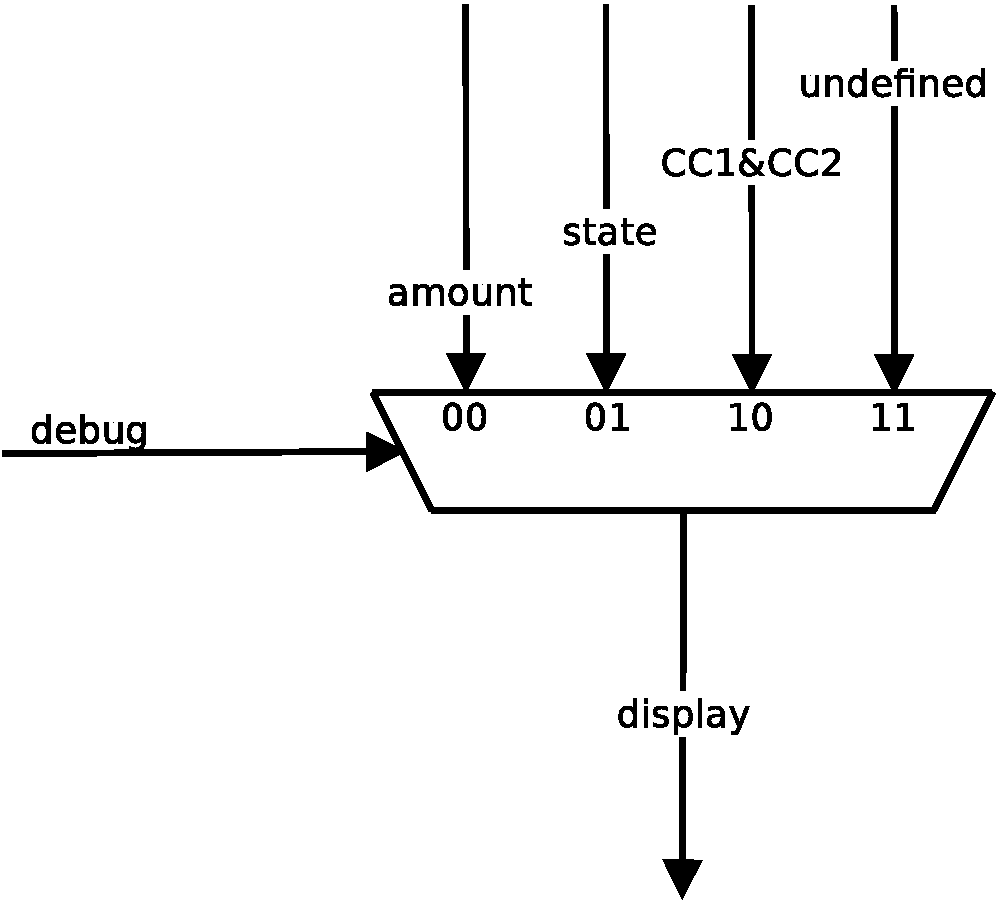
\includegraphics[width=0.3\textwidth]{fig/datapath_debug.pdf}
\caption{Datapath of the debug circuit}
\label{fig:debug}
\end{figure}

\subsection{Implementation issues}
\label{sec:implementation_issues}
\subsubsection{The missing coins}
\label{sec:missing_coins}
In our implementation we have a problem regarding input of coins. If a user were to insert a coin in a wrong state, for example insert a 2 kr in the add1 state, this input would be lost, thus "eating" the users coins.\\
This was tried resolved in the project by reacting to kr1 and kr2 inputs in the add2 and add1 respectively. This proved unsuccessful, as we would introduce the opportunity of inserting more than 8 kr in the machine. This would imply that that the user would have to insert money in every clock cycle. We decided that the first problem was the lesser of several evils, as it would probably not pose a problem when using a fast clock.